%%% Preamble
\documentclass[paper=a4, fontsize=11pt]{scrartcl}

\usepackage[english]{babel}	
\usepackage{tikz}
\usepackage{pgfplots}
\pgfplotsset{compat=1.15}

%%% Custom sectioning
\usepackage{sectsty}
\allsectionsfont{\centering \normalfont\scshape}

%%% Begin document
\begin{document}
\section{Labwork 3 : First step of Cuda}

    
    The code :
    \begin{verbatim}
    __global__ void grayscale(uchar3 *input, uchar3 *output) {
        int tid = threadIdx.x + blockIdx.x * blockDim.x;
        output[tid].x = (input[tid].x + input[tid].y +
        input[tid].z) / 3;
        output[tid].z = output[tid].y = output[tid].x;
    }
	
void Labwork::labwork3_GPU() {

	// Get the basic variable such as the pixelcount block size etc ..
	int pixelCount = inputImage->width * inputImage->height;
	int blockSize = 64;
	int numBlock = pixelCount / blockSize;

	
	uchar3 *devInput;
	uchar3 *devGray;
	
	// Initialize the output image
	outputImage = static_cast<char *>(malloc(pixelCount * 3));
	
	// Allocate the memory in the device for the Deviceinput and the Deviceouput
	cudaMalloc(&devInput, pixelCount * sizeof(uchar3));
	cudaMalloc(&devGray, pixelCount * sizeof(uchar3));
	
	// Copy from the HostInput to the devInput (here, the image)
	cudaMemcpy(devInput, inputImage->buffer,pixelCount * sizeof(uchar3),cudaMemcpyHostToDevice);
	
	// Do the thing you want to do
	grayscale<<<numBlock, blockSize>>>(devInput, devGray);
	
	// Copy from the DeviceOutput to the HostOutput (here the image in grayscale)
	cudaMemcpy(outputImage, devGray,pixelCount * sizeof(uchar3),cudaMemcpyDeviceToHost);
	
	// Don't forget to free
	cudaFree(devInput);
	cudaFree(devGray);

}
    \end{verbatim}
    
    First, we initialize the basic settings of our image, the number of pixels, the size and the number of blocks.Then, we allocate the memory that DevInput and DevOutput will use, using the cudaMalloc function. We can now copy the image (Basically the HostInput) from inputImageBuffer to our freshly allocated devInput variable using cudamemecpy. The device can now execute the grayscale Kernel on the image. The output of the operation will be store in devGray (DevOutput). Using cudaMemecpy we can copy the data from devGray to our output Image. Don't forget to free devInput and devGray, we won't use those anymore.\newline
    
    The output : ( labwork 1 vs labwork 2 )
    
    \begin{verbatim}
    USTH ICT Master 2018, Advanced Programming for HPC.
	Warming up...
	Starting labwork 1
	labwork 1 CPU ellapsed 3179.9ms
	labwork 1 OpenMP ellapsed 813.1ms

    ___________________________________________
    USTH ICT Master 2018, Advanced Programming for HPC.
    Warming up...
    Starting labwork 3
    labwork 3 ellapsed 82.0ms

    \end{verbatim}
    
    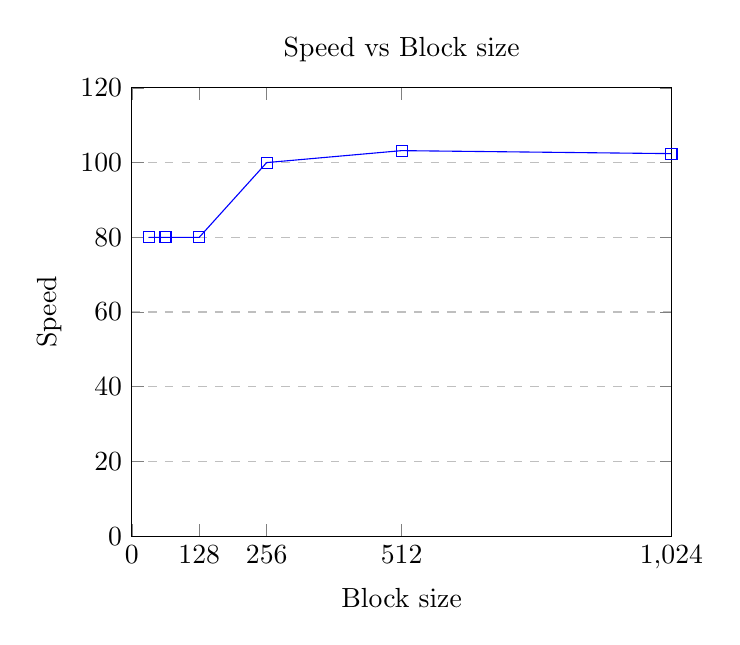
\begin{tikzpicture}

\begin{axis}[
    title={Speed vs Block size},
    xlabel={Block size},
    ylabel={Speed},
    xmin=0, xmax=1024,
    ymin=0, ymax=120,
    xtick={0,128,256,512,1024},
    ytick={0,20,40,60,80,100,120},
    legend pos=north west,
    ymajorgrids=true,
    grid style=dashed,
]
 
\addplot[
    color=blue,
    mark=square,
    ]
    coordinates {
    (32,80)(64,80)(128,80)(256,100)(512,103.2)(1024,102.4)
    };
 
\end{axis}
\end{tikzpicture}
%%% End document
\end{document}
